\section{Van Der Pol Example}
\label{Van Der Pol Example}




\begin{figure}[h]
    \centering
    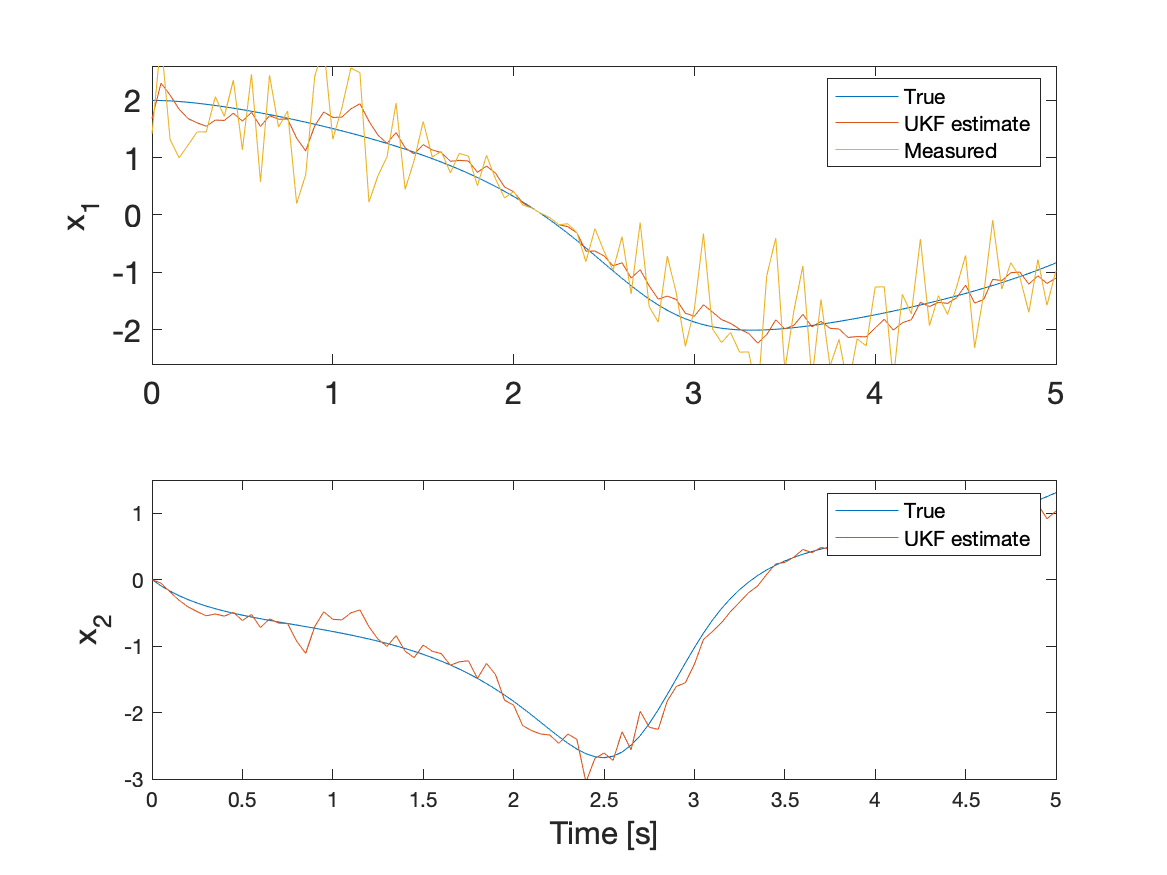
\includegraphics[scale = 0.6]{VDP.png}
    \caption{Optimized UKF for VDP oscillator}
    \label{map}
\end{figure}

\begin{figure}[!tbp]
  \centering
  \subfloat[UKF with high measurement noise]{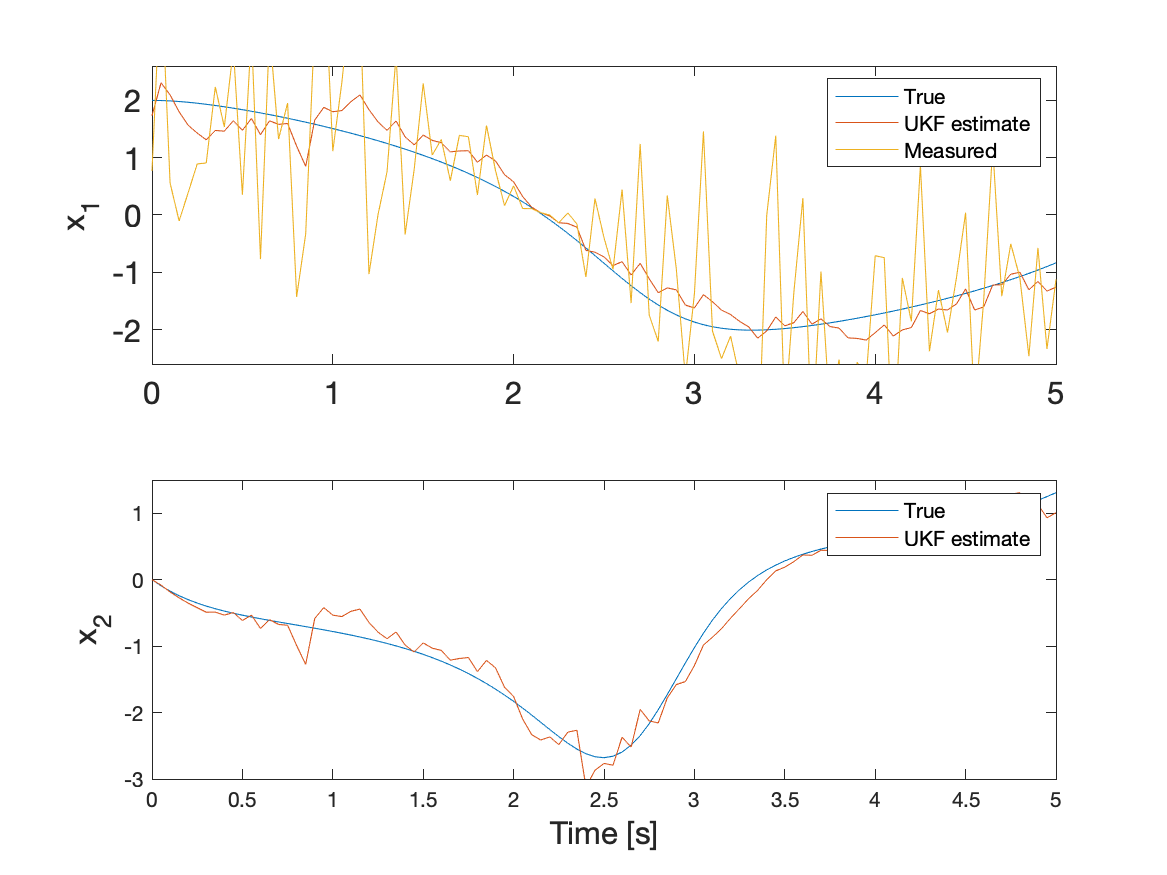
\includegraphics[width=0.5\textwidth]{VDP_highMN.png}\label{fig:f1}}
  \hfill
  \subfloat[UKF with low measurement noise]{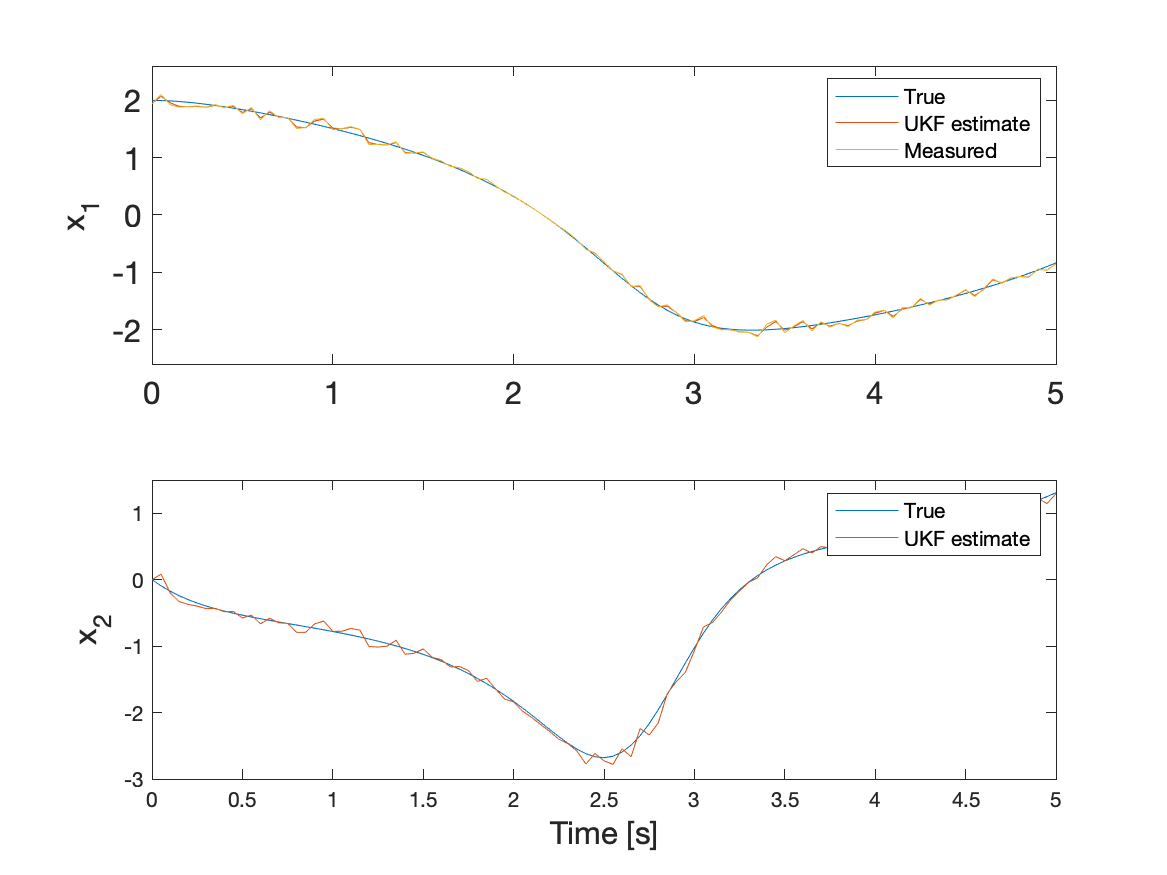
\includegraphics[width=0.5\textwidth]{VDP_lowMN.png}\label{fig:f2}}
  \caption{UKF on VDP oscillator differences in measurement noise.}
\end{figure}

\begin{figure}[!tbp]
  \centering
  \subfloat[UKF with high process noise]{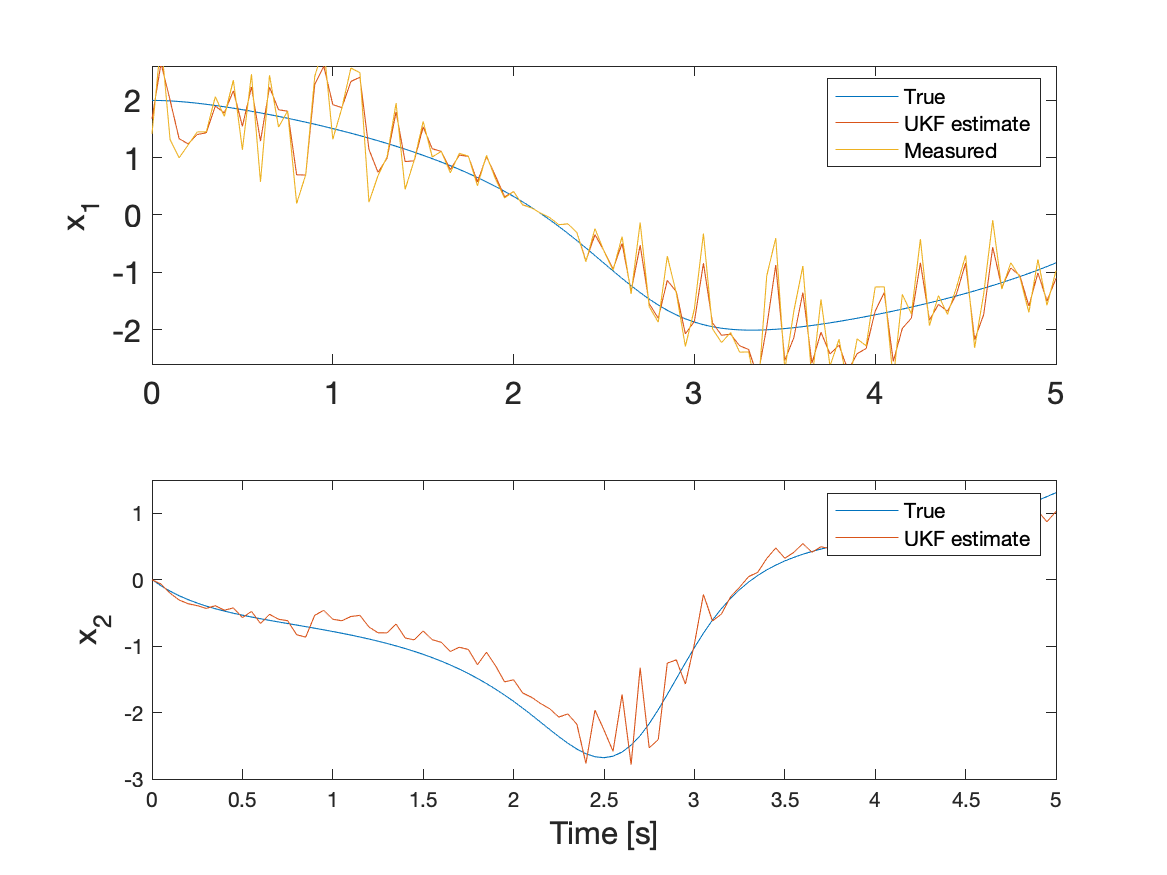
\includegraphics[width=0.5\textwidth]{VDP_highPN.png}\label{fig:f1}}
  \hfill
  \subfloat[UKF with low process noise]{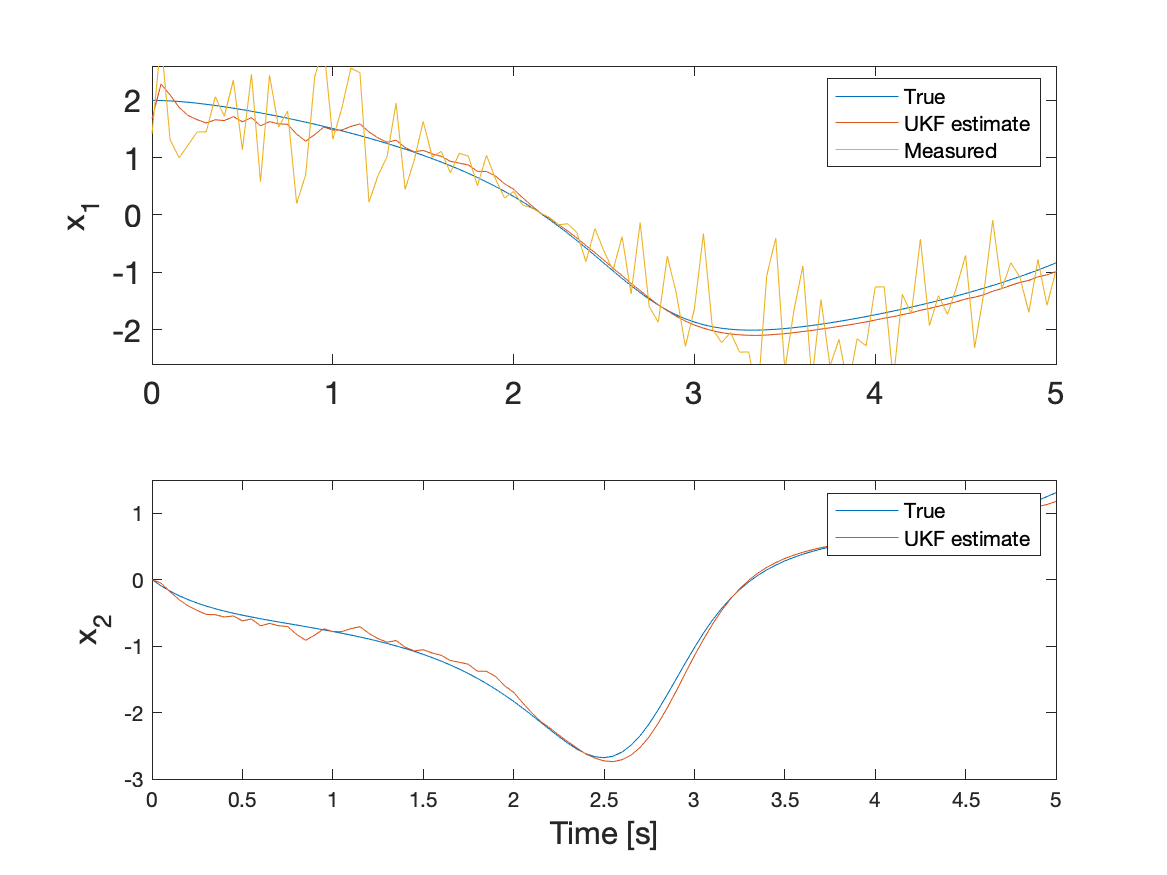
\includegraphics[width=0.5\textwidth]{VDP_lowPN.png}\label{fig:f2}}
  \caption{UKF on VDP oscillator differences in process noise.}
\end{figure}